% arara: latex: { interaction: nonstopmode, options: ['-halt-on-error'] }
% arara: dvisvgm: { options: ['--no-fonts', '--exact-bbox', '--zoom=-1'] }
% Both collinear orders are needed. C is the third-loop disk.
% Left: C_prev is the second-loop disk immediately before P_j was tested.
% Right: C_prev is the first-loop disk immediately before P_i was tested.
% In each case the previously covered segment also covers the tested point,
% contradicting the outside test that was required to trigger the rebuild.
\documentclass[tikz,border=8pt,11pt]{standalone}
\usepackage{amsmath,amssymb}
\definecolor{circleblue}{HTML}{0072B2}
\definecolor{pointred}{HTML}{D55E00}
\definecolor{fixedpurple}{HTML}{8B4C9D}
\definecolor{ink}{HTML}{25313C}
\definecolor{muted}{HTML}{7C8792}
\tikzset{
  current/.style={draw=circleblue,line width=1.1pt,fill=circleblue!5},
  previous/.style={draw=muted,dashed,line width=0.9pt},
  point label/.style={inner sep=2pt,fill=white},
}
\newcommand{\fixedpoint}[3]{%
  \fill[ink] (#1,#2) circle[radius=2.3pt];
  \draw[fixedpurple,line width=1.1pt] (#1,#2) circle[radius=5pt];
  \node[point label,below=6pt] at (#1,#2) {$#3$};
}
\begin{document}
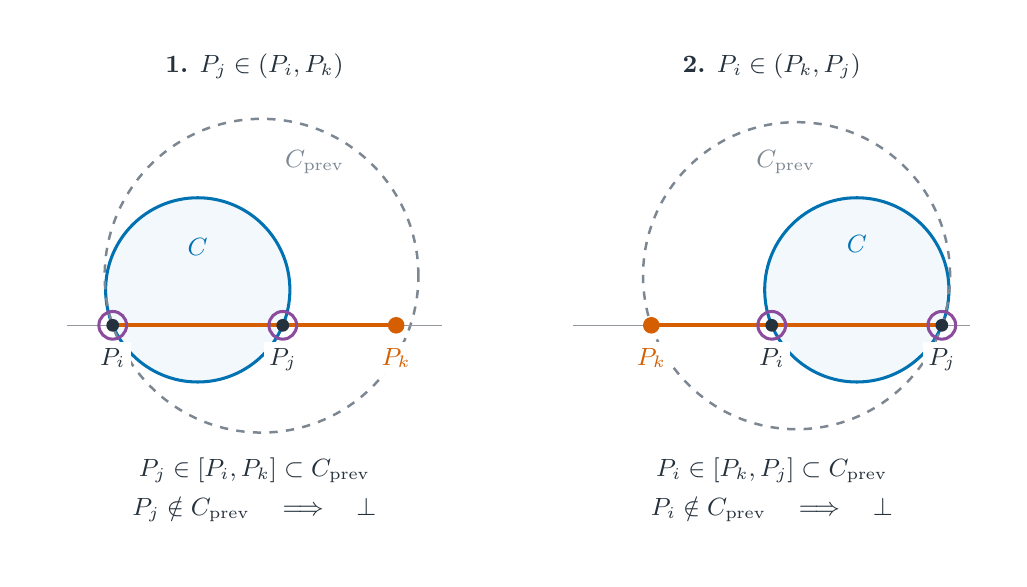
\begin{tikzpicture}[x=0.9cm,y=0.9cm,font=\small,text=ink]
  \fill[white] (-3.2,-3.3) rectangle (10.5,4.2);

  \begin{scope}
    \node at (0,3.65) {\textbf{1.} $P_j\in(P_i,P_k)$};
    % C: center (-0.8,0.5), radius 1.3; horizontal chord [-2,0.4].
    % C_prev: center (0.1,0.7), radius sqrt(4.9); chord [-2,2.2].
    \draw[current] (-0.8,0.5) circle[radius=1.3];
    \draw[previous] (0.1,0.7) circle[radius={sqrt(4.9)}];
    \draw[ink!50] (-2.65,0) -- (2.65,0);
    \draw[pointred,line width=1.5pt] (-2,0) -- (2,0);
    \fixedpoint{-2}{0}{P_i}
    \fixedpoint{0.4}{0}{P_j}
    \fill[pointred] (2,0) circle[radius=3pt];
    \node[point label,below=6pt,text=pointred] at (2,0) {$P_k$};
    \node[text=circleblue] at (-0.8,1.1) {$C$};
    \node[text=muted] at (0.85,2.3) {$C_{\mathrm{prev}}$};
    \node at (0,-2.05) {$P_j\in[P_i,P_k]\subset C_{\mathrm{prev}}$};
    \node at (0,-2.6) {$P_j\notin C_{\mathrm{prev}}\quad\Longrightarrow\quad\bot$};
  \end{scope}

  \begin{scope}[xshift=6.57cm]
    \node at (0,3.65) {\textbf{2.} $P_i\in(P_k,P_j)$};
    % C: center (1.2,0.5), radius 1.3; horizontal chord [0,2.4].
    % C_prev: center (0.35,0.7), radius sqrt(4.6925); chord [-1.7,2.4].
    \draw[current] (1.2,0.5) circle[radius=1.3];
    \draw[previous] (0.35,0.7) circle[radius={sqrt(4.6925)}];
    \draw[ink!50] (-2.8,0) -- (2.8,0);
    \draw[pointred,line width=1.5pt] (-1.7,0) -- (2.4,0);
    \fixedpoint{0}{0}{P_i}
    \fixedpoint{2.4}{0}{P_j}
    \fill[pointred] (-1.7,0) circle[radius=3pt];
    \node[point label,below=6pt,text=pointred] at (-1.7,0) {$P_k$};
    \node[text=circleblue] at (1.2,1.15) {$C$};
    \node[text=muted] at (0.2,2.3) {$C_{\mathrm{prev}}$};
    \node at (0,-2.05) {$P_i\in[P_k,P_j]\subset C_{\mathrm{prev}}$};
    \node at (0,-2.6) {$P_i\notin C_{\mathrm{prev}}\quad\Longrightarrow\quad\bot$};
  \end{scope}
\end{tikzpicture}
\end{document}
